\documentclass[10pt,a4paper]{report}
\usepackage[latin1]{inputenc}
\usepackage{amsmath}
\usepackage{amsfonts}
\usepackage{amssymb}
\usepackage{graphicx}
\author{Seth Bertlshofer\\Alexis Tyler\\Dustin Ginos\\Kevin Burgon}
\title{Desc. Experience 1}
\graphicspath{{img/}}
\begin{document}
	\maketitle
	\textbf{Sub-Experience One: Fun and Games}\\
		\begin{center}
			Figure 1.\\
			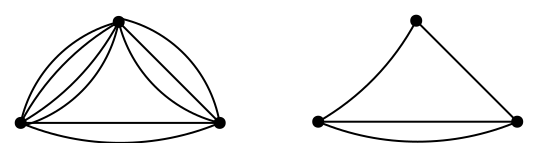
\includegraphics[scale=.5]{e1.png}
			\newline
			\newline
		\end{center}

	\textbf{Sub-Experience Two: The Binary Addressing Graph}
		\begin{enumerate}
			\item $|V(Q_n)| = 2^n$
			\begin{center}
				Figure 2.\\
				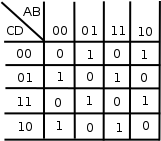
\includegraphics[scale=.5]{2_1.png}
			\end{center}
			Because this solution is looking for a binary power we can prove this with a Karnaugh Map (Figure 2) What this shows in the relation between the vertices.  If there is a relation then 1's will be adjacent to one another.  We can see that because the pattern is that is created by the Karnaugh map there can be no relations between vertices.
			\item $Q_n$ is an n-regular graph: that is, $deg (\vec{v}) = n $ for each $\vec{v} \epsilon V(Q_n)$.
			\item $Q_n$ is \textit{bipartite}; that is, $V(Q_n)$ consists of two sets, say X and Y such that $X\cap Y = \varnothing$ and the only edges of $Q_n$ have one end-vertex in X and the other in Y (so X and Y induce graphs with no edges).
			\item $Q_n$ is Hamiltonian for $n \geq 2$.
		\end{enumerate}
		
		
	\textbf{Sub-Experience Three: Space Station Problems}\\
	
		\begin{center}
			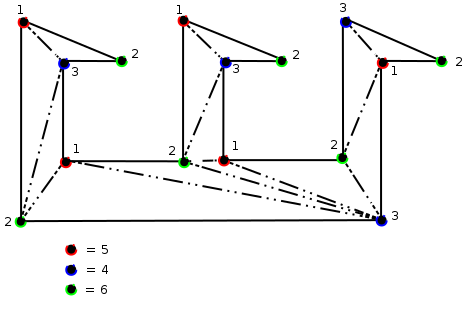
\includegraphics[scale=.5]{e3.png}
			\newline
			\newline
		\end{center}
	\textbf{Sub-Experience Four: Regions Determined by Chords of a Circle}\\
	
		\begin{center}
			%\includegraphics[scale=.5]{.png}
	
		\end{center}
	\textbf{Sub-Experience Five: Survivors in a Tournament.}\\
	
		\begin{center}
			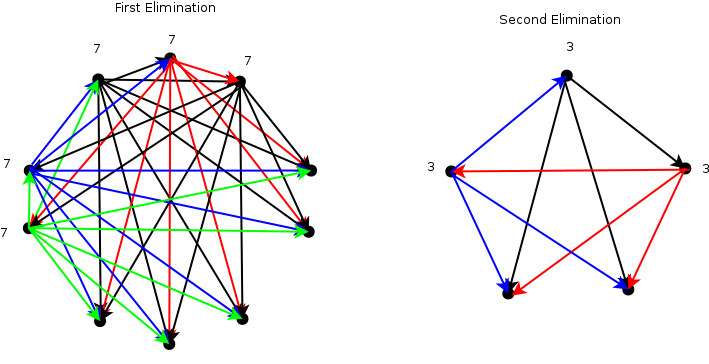
\includegraphics[scale=.5]{e5.png}
			\newline
			\newline
		\end{center}
	\textbf{Sub-Experience Six: Better-Than-Good Will Hunting}\\
		Verify that the graph G (below) has a diameter of 2.
	
		By using Lemma 2 we can prove that this graph does indeed have a diameter of 2.  
		\begin{center}
			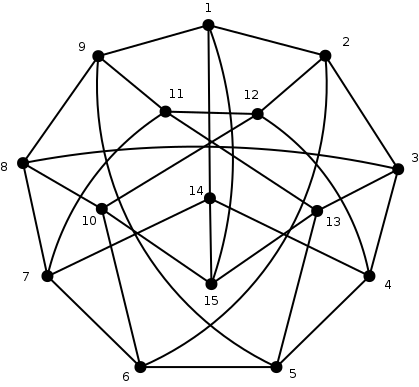
\includegraphics[scale=.5]{e6.png}
			\newline
			\newline
		\end{center}
	\textbf{[Bonus] Sub-Experience Seven: A Matter of Life and Death}\\	
	
		\begin{center}
			%\includegraphics[scale=.5]{.png}

		\end{center}
\end{document}